\documentclass[]{report}
\usepackage{graphicx, float,}
\usepackage{hyperref}
\usepackage[export]{adjustbox}

\title{\centering CSD300 : Design Project \\Music Genre Recognition}
\author{\LARGE Vaibhav Vashisht\\ \LARGE 2016UCS0002\\ \\ \LARGE Sahil\\ \LARGE 2016UCS0008}

% to use proper section numbering in the report type 
\renewcommand{\thesection}{\arabic{section}}

\begin{document} 

\maketitle

%%%%%%%%%%%%%%%%%%%%%%%%%%%%%%%%%%%%%%%%%%%%%%%%
\section{Problem Statement:}
\large Wikipedia defines music genre as a conventional category that identifies pieces of
music as belonging to a shared tradition or set of conventions. Classifying songs
according to genre is something that has been till now done by human tagging.
The necessity for such a tagged dataset arises for any music search engine that
aims to suggest similar songs to the user. Characteristics that define a song to
be in a particular genre are usually somewhat abstract and often a song may
have overlapping genres. To automate the task of genre classification one first
needs a suitable feature vector to represent the song. We aim to classify genre
independent of the metadata (artist information, lyrics etc).

\section{Methodology:}
\large 
Here’s a general overview of what we will do:
\begin{itemize}
	\item Extract a simplified representation of the songs (.wav file).
	\item Train a neural network to classify the songs.
	\item Use the classifier to find the genre.
\end{itemize}

\begin{figure}[H]
	\vspace{0pt}
	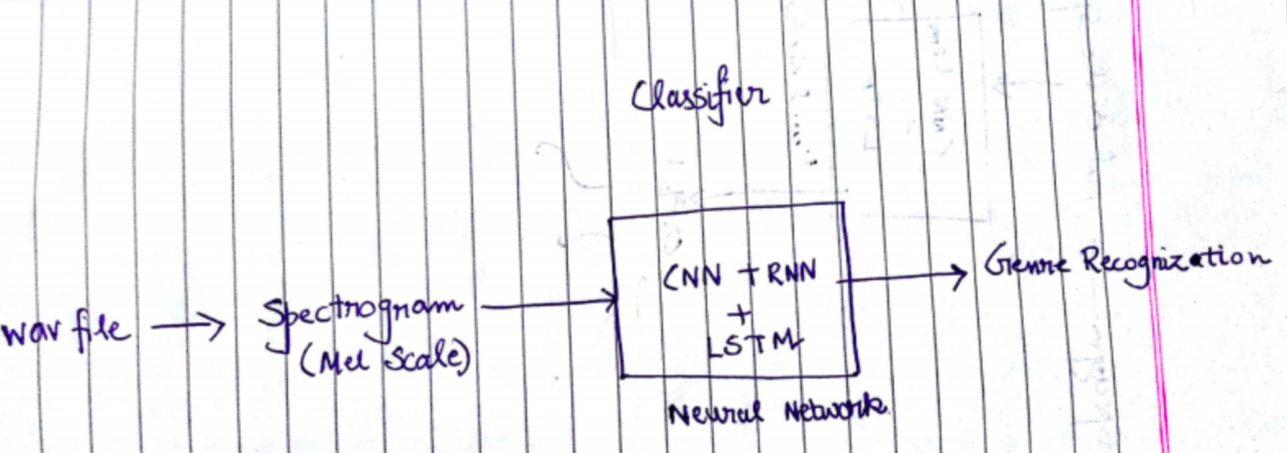
\includegraphics[height = 150pt, keepaspectratio]{method.png}
\end{figure}

\section{Tools/softwares required:}
\begin{itemize}
	\item \textbf{Librosa:} is a python package for music and audio analysis.
	\item \textbf{PyTorch or Keras:} for neural networks. 
	\item \textbf{Google Colab:} for training the model on GPU. 
	
\end{itemize}
\section{Data collection:}
This dataset was used for the well known paper in genre classification ”Musical
genre classification of audio signals” by G. Tzanetakis and P. Cook in IEEE
Transactions on Audio and Speech Processing 2002. The dataset consists of
1000 audio tracks each 30 seconds long. It contains 10 genres, each represented
by 100 tracks. The tracks are all 22050Hz Mono 16-bit audio files in .wav format.

\end{document}